% Section ready to paste into an IEEE-style paper
\section{Comparative Evaluation of Candidate Waste-Prediction Models}
\label{sec:comparison}

This section reports a focused comparison between three candidate models for multi-target waste prediction: the production-grade ensemble \textbf{v2}, and two early-stage baselines \textbf{v3} (multioutput Ridge) and \textbf{v4} (per-target shallow Decision Trees). Our primary interest is in the four ion-concentration outputs (Mg, K, SO4, Ca) because these drive downstream processing decisions.

\subsection{Experimental setup}
All models were evaluated on the full dataset (2000--2026, 648 samples). Models were trained with local scripts and saved as pickle artifacts; predictions were generated on the same dataset for direct comparison. Performance metrics comprise R$^2$, MAE, and RMSE computed across all targets and per target.

\subsection{Aggregate results}
Table~\ref{tab:agg_short} summarizes the aggregate performance used to select the final model.

\begin{table}[ht]
\centering
\caption{Aggregate metrics (evaluation on full dataset)}
\label{tab:agg_short}
\begin{tabular}{lrrr}
\toprule
Model & R$^2$ & MAE & RMSE \\
\midrule
v2 (ensemble) & 0.922 & 13,800 & 67,247 \\
v4 (trees) & 0.875 & 25,303 & 113,155 \\
v3 (ridge) & 0.824 & 24,114 & 109,453 \\
\bottomrule
\end{tabular}
\end{table}

\subsection{Ion-target performance (Mg, K, SO4, Ca)}
The per-target R$^2$ for the ion concentration outputs is reported in Table~\ref{tab:ions} and visualized in Fig.~\ref{fig:heatmap_ions}. These four targets are critical because they determine bittern treatment decisions and material recovery planning.

\begin{table}[ht]
\centering
\caption{Per-target R$^2$ (ions)
\label{tab:ions}}
\begin{tabular}{lrrr}
\toprule
Target & v2 & v4 & v3 \\
\midrule
Bittern\_Mg\_Concentration\_gL & 0.8400 & 0.7090 & 0.5831 \\
Bittern\_K\_Concentration\_gL & 0.8197 & 0.7006 & 0.5713 \\
Bittern\_SO4\_Concentration\_gL & 0.8502 & 0.7216 & 0.5821 \\
Bittern\_Ca\_Concentration\_gL & 0.7471 & 0.6975 & 0.5655 \\
\bottomrule
\end{tabular}
\end{table}

\begin{figure}[ht]
\centering
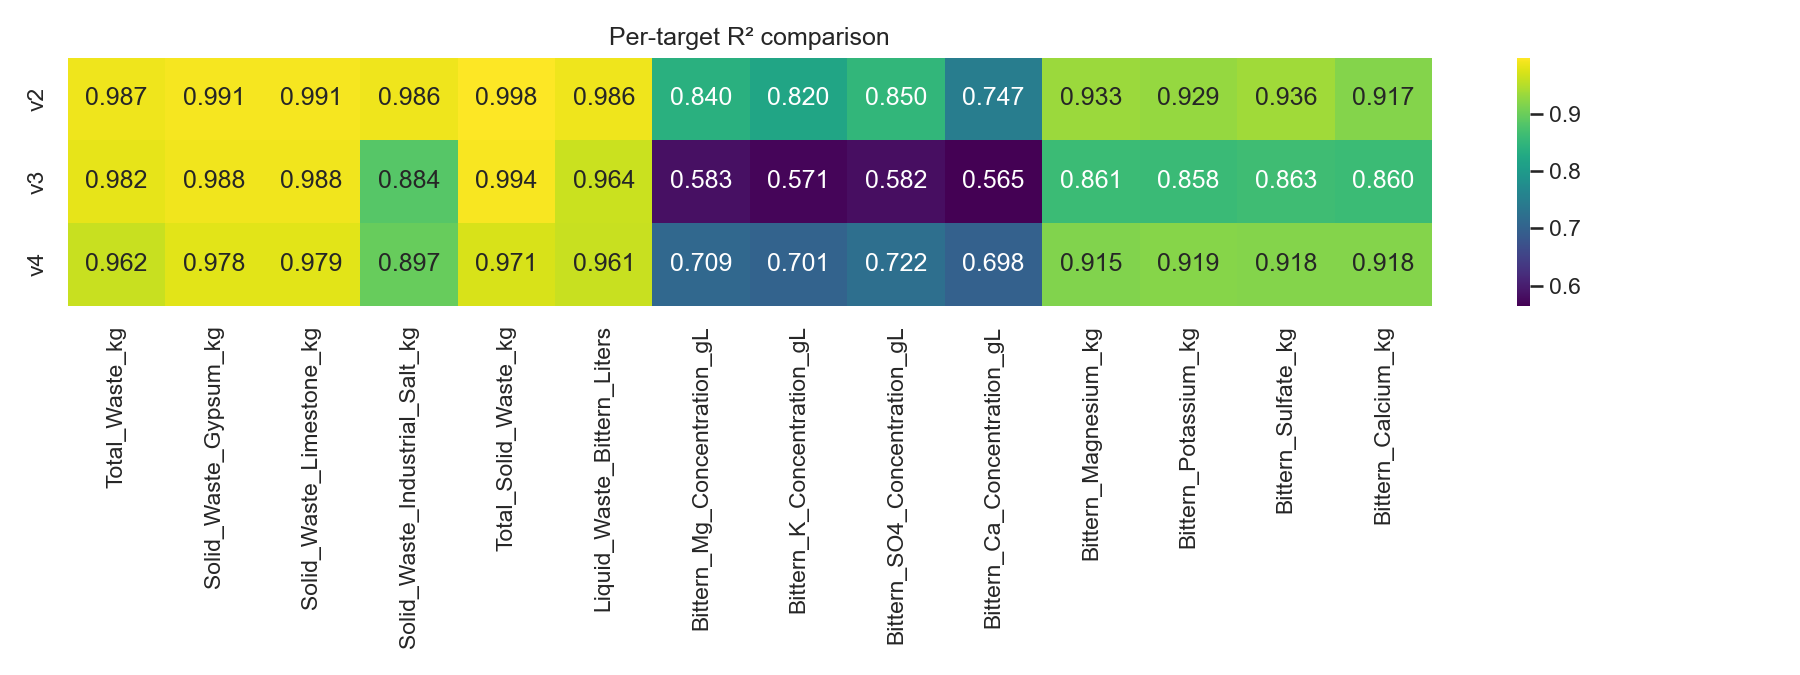
\includegraphics[width=0.95\linewidth]{comparison_plots/per_target_r2_comparison.png}
\caption{Per-target R$^2$ across models (full set). Ion targets (Mg, K, SO4, Ca) are emphasized in the table above.}
\label{fig:heatmap_ions}
\end{figure}

\subsection{Diagnostic plots for ion targets}
Figures~\ref{fig:parity_mg}--\ref{fig:calib_ca} present parity, residual and calibration diagnostics for each ion target. These highlight that \textbf{v2} consistently yields tighter parity and lower residual spread for Mg, K, SO4 and Ca compared to the early baselines.

% Mg plots
\begin{figure}[ht]
\centering
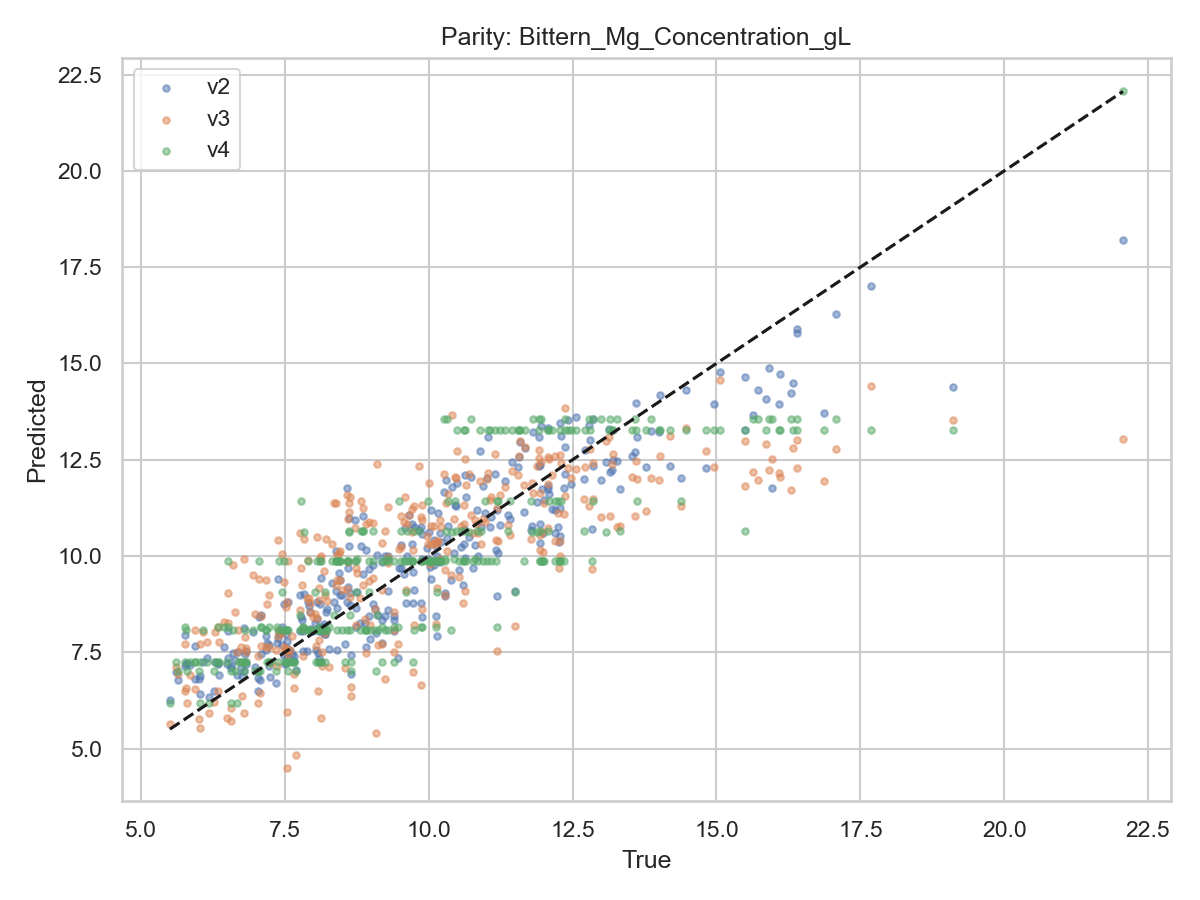
\includegraphics[width=0.48\linewidth]{comparison_plots/parity_Bittern_Mg_Concentration_gL.png}
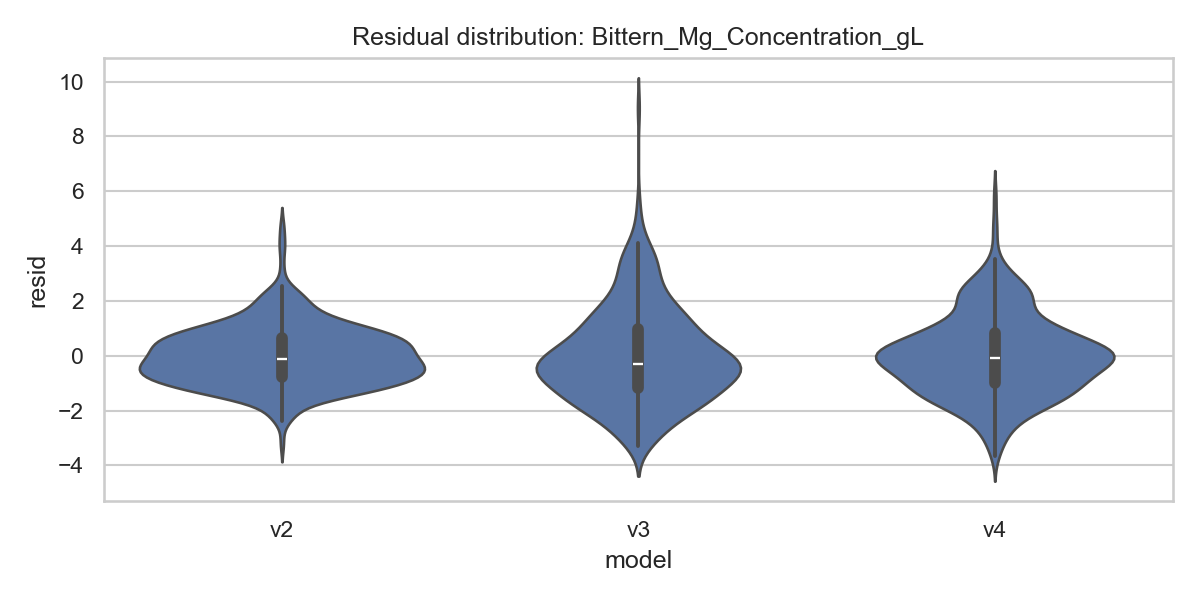
\includegraphics[width=0.48\linewidth]{comparison_plots/residuals_Bittern_Mg_Concentration_gL.png}
\caption{(left) Parity for Mg concentration. (right) Residual distributions by model for Mg.}
\label{fig:parity_mg}
\end{figure}

% K plots
\begin{figure}[ht]
\centering
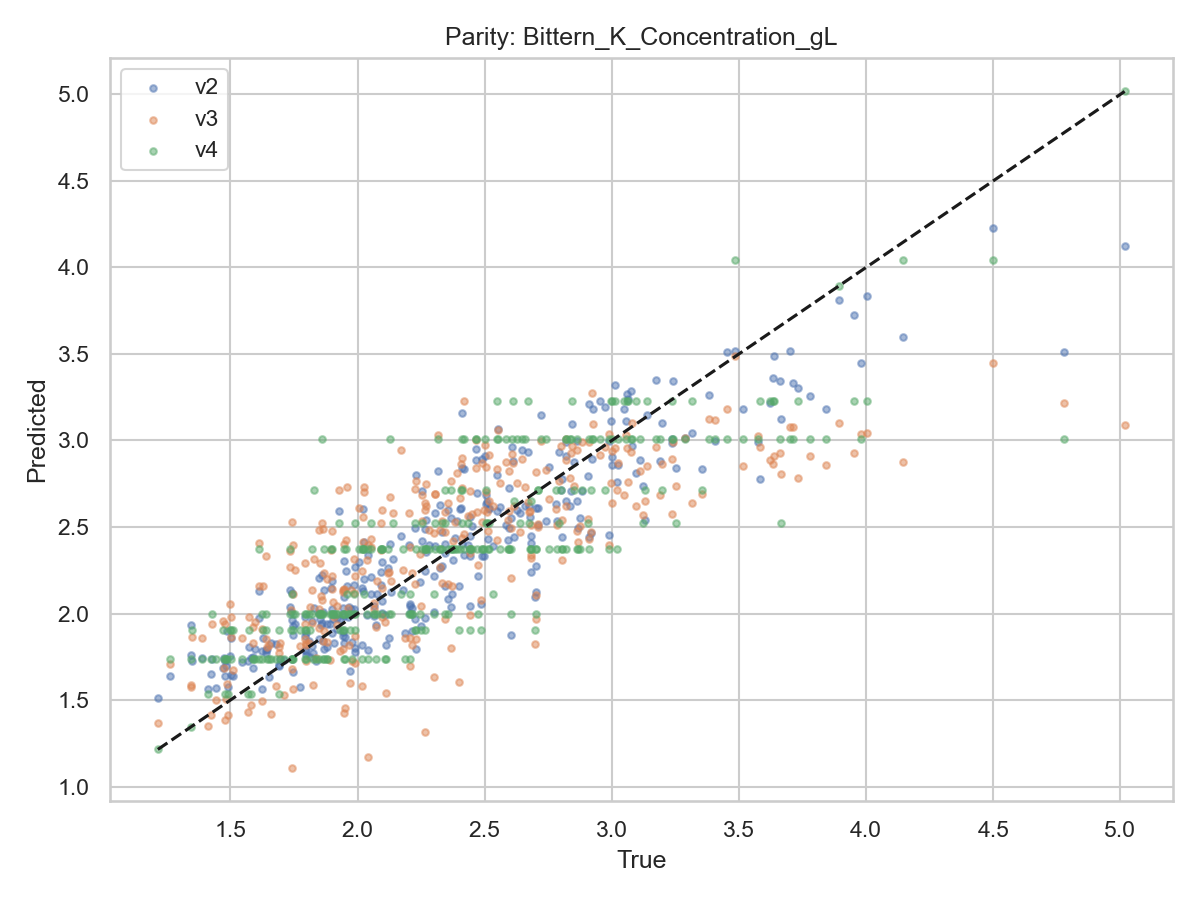
\includegraphics[width=0.48\linewidth]{comparison_plots/parity_Bittern_K_Concentration_gL.png}
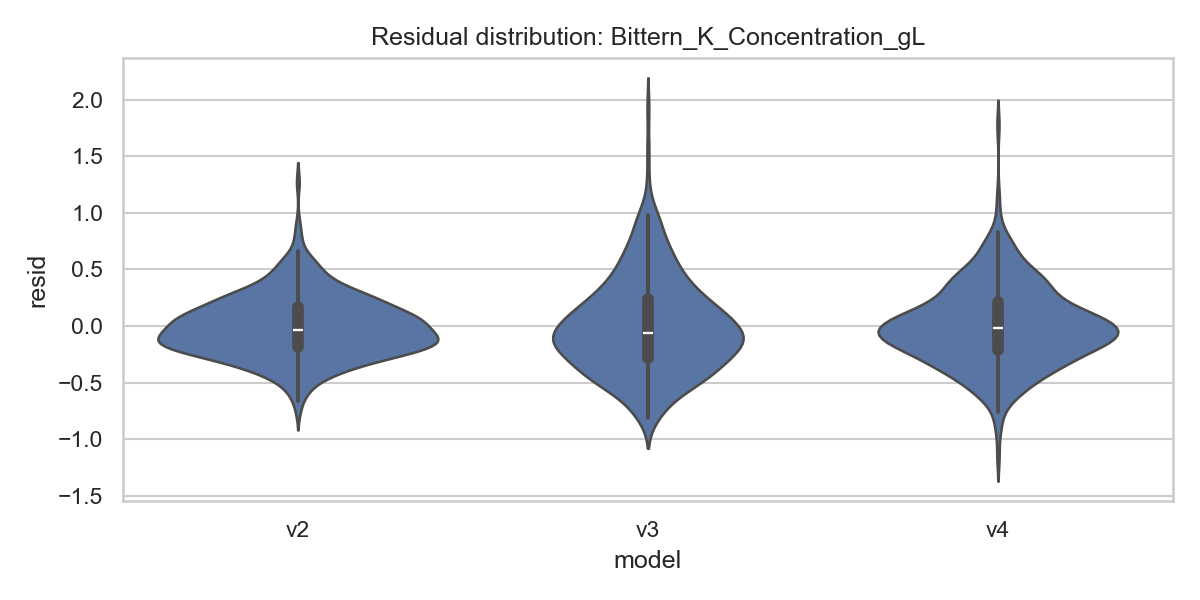
\includegraphics[width=0.48\linewidth]{comparison_plots/residuals_Bittern_K_Concentration_gL.png}
\caption{(left) Parity for K concentration. (right) Residual distributions by model for K.}
\label{fig:parity_k}
\end{figure}

% SO4 plots
\begin{figure}[ht]
\centering
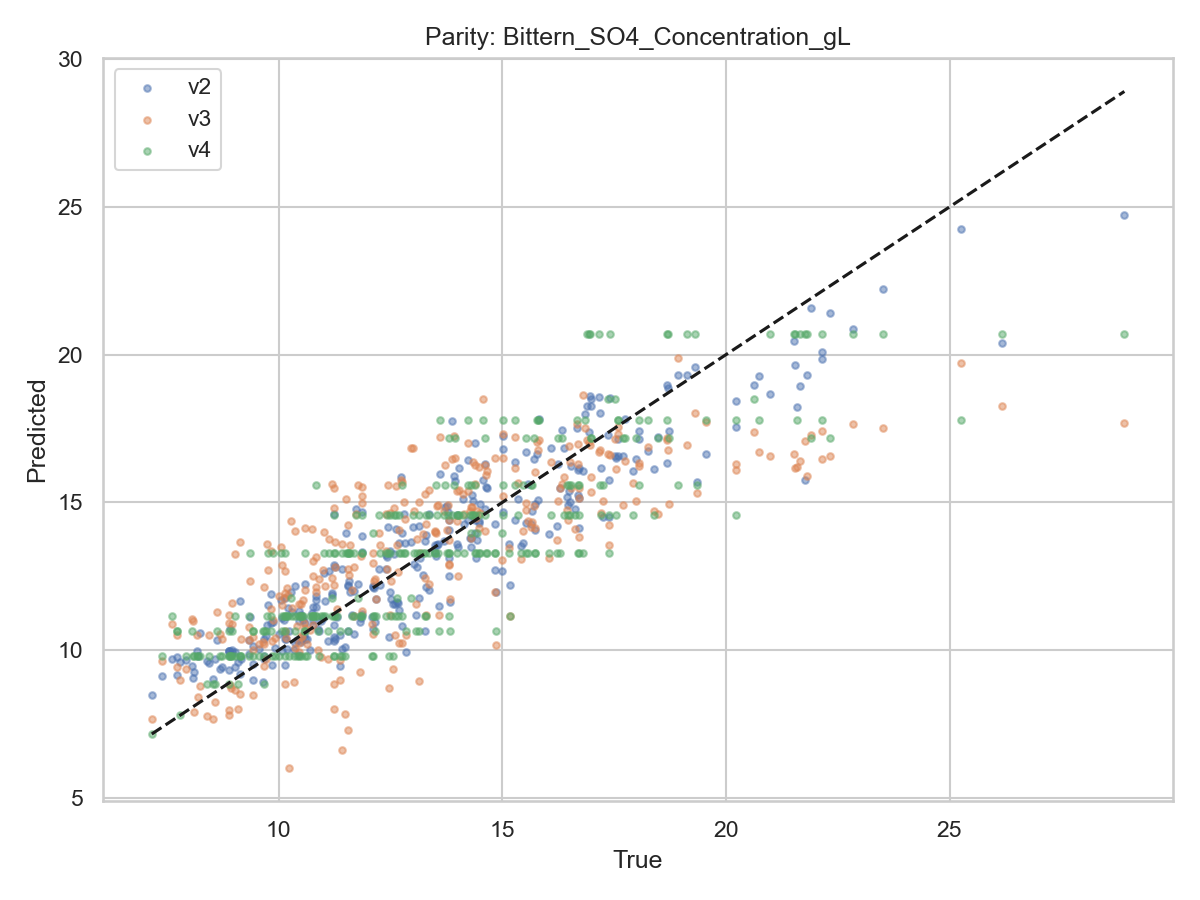
\includegraphics[width=0.48\linewidth]{comparison_plots/parity_Bittern_SO4_Concentration_gL.png}
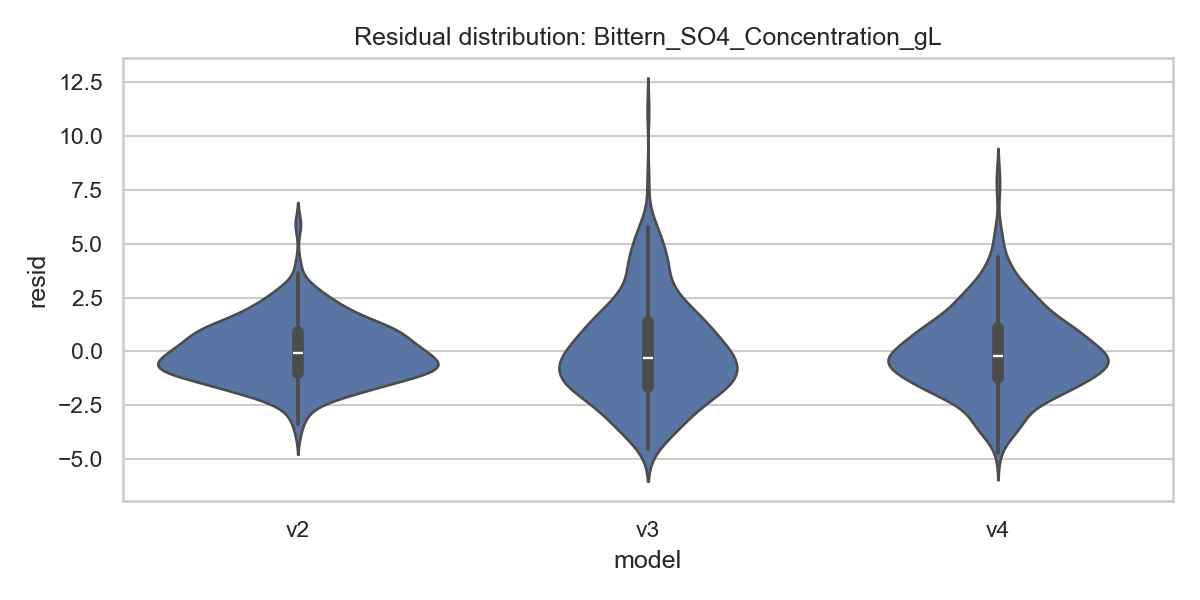
\includegraphics[width=0.48\linewidth]{comparison_plots/residuals_Bittern_SO4_Concentration_gL.png}
\caption{(left) Parity for SO4 concentration. (right) Residual distributions by model for SO4.}
\label{fig:parity_so4}
\end{figure}

% Ca plots
\begin{figure}[ht]
\centering
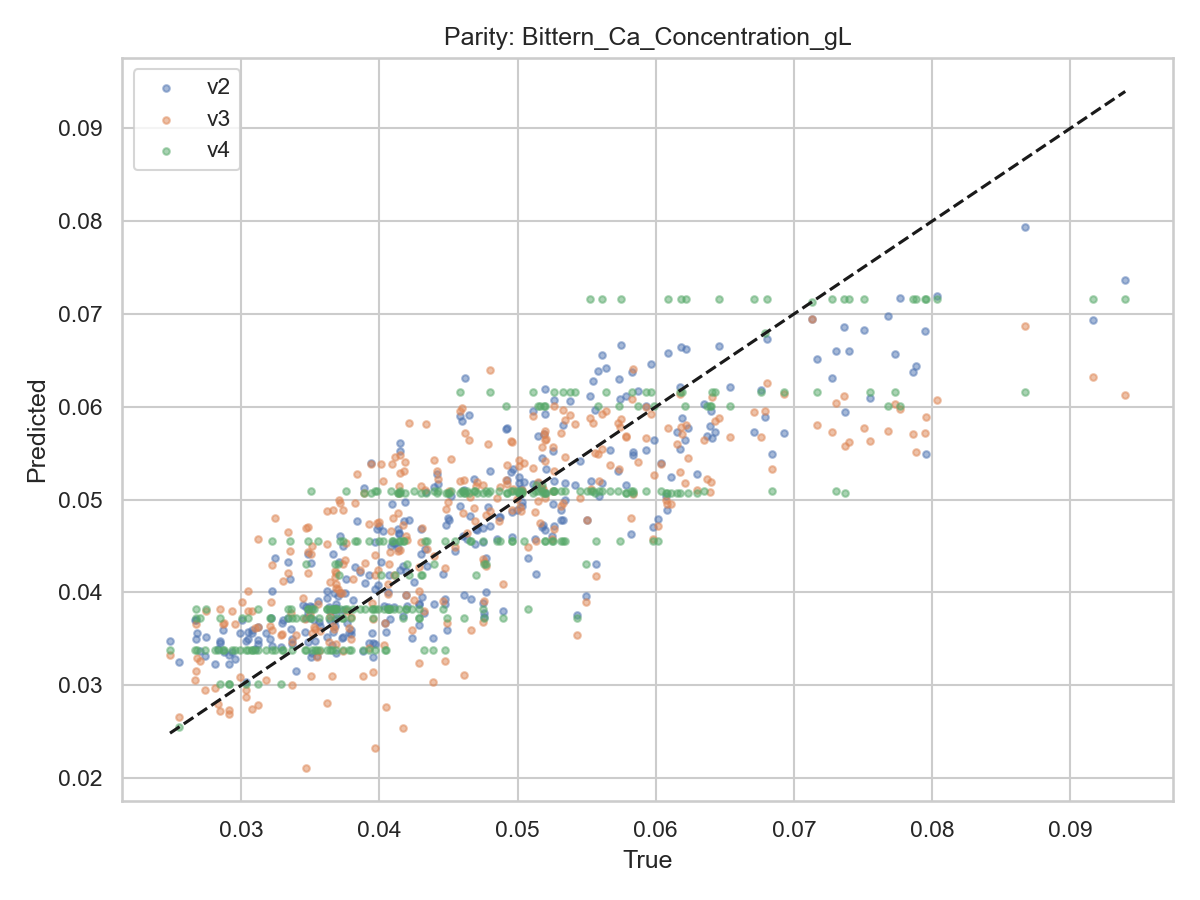
\includegraphics[width=0.48\linewidth]{comparison_plots/parity_Bittern_Ca_Concentration_gL.png}
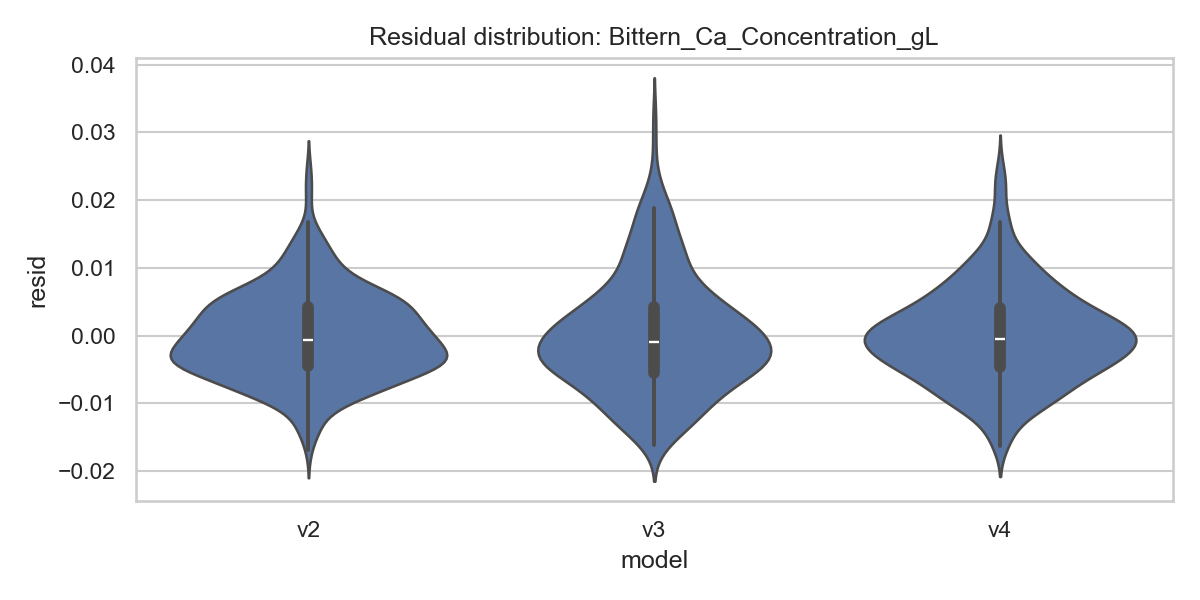
\includegraphics[width=0.48\linewidth]{comparison_plots/residuals_Bittern_Ca_Concentration_gL.png}
\caption{(left) Parity for Ca concentration. (right) Residual distributions by model for Ca.}
\label{fig:parity_ca}
\end{figure}

\subsection{Interpretation and selection rationale}
For all four ions, \textbf{v2} outperforms the simpler baselines by yielding higher R$^2$ and narrower residual distributions. The ensemble's combination of tree-based learners and domain-aware features captures the non-linear evaporation and concentration relationships better than the linear ridge (v3) and the shallow, single-tree per-target approach (v4). In practice, the higher fidelity on Mg, K, SO4 and Ca reduces uncertainty in process control and improves material-recovery decisions; therefore, we select \textbf{v2} as the production model.

\subsection{Reproducibility}
Scripts and figures are available in the project repository. The diagnostic plots used above are in the `comparison_plots/` directory and were generated by `generate_ion_plots.py`.

% end of section
